

\subsection{Modelos Matem\'aticos \emph{Depredador-Presa}}

El uso de modelos matem\'aticos para describir la din\'amica poblacional de un conjunto de especies que se relacionan mediante interacciones depredador-presa, se remonta a los trabajos de Lotka y Volterra\citep{gotelliprimer}, los cuales independientemente describieron los cambios en la abundancia poblacional de un depredador $C$ y una presa $R$ mediante el siguiente sistema de ecuaciones diferenciales : 

\begin{equation}\label{eq:LV}
\begin{aligned}
&\dot{R} = R(r - \alpha C)\\
&\dot{C} = C(e\alpha - q) 
\end{aligned}
\end{equation}

El sistema \eqref{eq:LV} es conocido como \emph{sistema de ecuaciones depredador-presa Lotka-Volterra} y se puede extender f\'acilmente a un sistema de $n$ especies identificadas con $\{1,2, \ldots ,n\}$ de la siguiente manera:
\begin{equation}\label{eq:LVGen}
\dot{X_i}  = X_i(b_i - d_i + \sum_{j}^n \alpha_{ij} X_j)
\end{equation}

Donde $X_i$ representa la abundancia en n\'umeros o biomasa de la especie $i$, $b_i$ la tasa intr\'inseca de producci\'on de masa(individuos), $d_i$ la tasa de p\'erdida de masa(individuos) y $\alpha_{ij}$ se puede interpretar como la p\'erdida(ganancia) de masa(individuos) debido a interacciones con las dem\'as especies presentes en el h\'abitat.

Por lo general se asume que :
\begin{itemize}
\item $\alpha_{ij}$ es una constante(la modificaci\'on $\alpha_{ij} = \alpha_{ij}(X)$ para una forma especf\'icia de la funci\'on da lugar a lo que se conoce como respuesta funcional tipo II  o tipo III).
\item $\alpha_{ii} < 0 $ si $X_i$ es un recurso basal, a diferencia de la formulaci\'on original en este caso se asume que existe \emph{denso dependencia directa} entre los individuos de una poblaci\'on de presas.
\item $\alpha_{ii} = 0 $ si $X_i$ es un depredador, es decir no existe \emph{denso dependencia directa} entre individuos de una poblaci\'on de depredadores, sin embargo la denso dependecia se da indirectamente a traves de la interacci\'on con los recursos..
\item $b_i = 0$ si $X_i$ es un depredador, ya que los depredadores no pueden subsistir en ausencia de presas.
\end{itemize}
Modelos como \eqref{eq:LVGen} son llamados \emph{modelos tipo Lotka-Volterra}.

El modelo depredador-presa \emph{Lotka-Volterra},pese a sus evidentes limitaciones,ha jugado(y sigue jugando) un papel importante en el desarrollo de la teor\'ia en ecolog\'ia y form\'o la base para el desarrollo de modelos que incorporan caracter\'isticas con mayor fundamento biol\'ogico. \\
Uno de los problemas que surge al momento de construir un modelo similar al de \eqref{eq:LVGen} es el como decidir \emph{a priori} el valor de los par\'ametros del modelo(e.g. $b_i , d_i$). Este problema se hace m\'as notorio conforme la dimensi\'on del modelo(i.e. n\'umero de ecuaciones en el sistema) crece \citep{yodzis1992body}.\\
Yodzis e Innes en su seminal paper \emph{Body size and Consumer-Resource dynamics}\citep{yodzis1992body} propusieron una forma para aligerar el problema.Ellos introdujeron lo que hoy en d\'ia se conoce como \emph{modelamiento bioenerg\'etico} el cual se basa en derivar los valores de los par\'ametros de las relaciones que existen entre ellos y la masa corporal, esta relaci\'on es generalmente de forma indirecta y se manifiesta debido a la influencia que tiene la masa sobre el metabolismo de las especies\citep{peters1986ecological}. A la fecha se han desarrollado diversos refinamientos a estas ideas, lo cual nos permite centrarnos en par\'ametros con mayor significado biol\'ogico.\citep{kiltie2000scaling,brown2004toward,savage2004predominance,pawar2012dimensionality,brose2010body}

\subsection{Ensamblaje}
En esta secci\'on definimos ciertos t\'erminos relacionados al proceso de ensamblaje de una comunidad. \\
Se denomina proceso de ensamblaje $E_A$ de una comunidad $A$ asociada a un h\'abitat $H$ al continuo de colonizaciones y extinciones de especies que se dan dentro de $H$, el conjunto de especies que \emph{potencialmente} puede colonizar a la comunidad $A$(i.e pueden por lo menos llegar a $H$) se denomina \emph{pool regional de especies}. 
\begin{equation}\label{eq:Assembly}
E_A := (A_0,H_0) \to (A_1,H_1) \to (A_2,H_2) \to \ldots
\end{equation}
En \eqref{eq:Assembly} cada cambio de $(A_i,H_i)$ a $(A_{i+1},H_{i+1})$ se da debido a un intento de colonizaci\'on sobre $(A_i,H_i)$,el cual puede tener uno de los tres siguientes desenlaces \citep{pawar2009community}: 
\begin{enumerate}
\item El invasor no puede invadir.
\item El invasor llega a invadir pero provoca extinciones en la comunidad receptora, pudiendo el mismo exintiguirse, esto es llamado \emph{invasi\'on inestable}.
\item El invasor llega a invadir y no provoca ninguna extinci\'on, esto es llamado \emph{invasi\'on estable}.
\end{enumerate}

De lo anterior se observa que la comunidad y h\'abitat f\'isico receptor juega un papel muy importante en el subsiguiente paso del proceso, adem\'as especificamos que cada estado $(A_i,H_i)$ puede estar en constante cambio,excepto por el n\'umero de especies, debido a la din\'amica inherente de las poblaciones de las especies presentes y por ende el tiempo entre distintas colonizaciones asu vez puede influenciar el desenlace de la colonizaci\'on debido a que la comunidad receptora puede estar en distintos estados(e.g. estado transiente $vs$ estado asint\'otico).\\

Sea $B = \{ (A_j,H_j) / j \in I, I \subseteq \mathbb{N}\}$ un conjunto de estados en $E_A$ , usando el formalismo definido en \eqref{eq:Assembly} decimos que la comunidad $A$ \emph{$\omega$-converge} a $B$ durante el ensamblaje si existe un $ m \in \mathbb{N}$ tal que $(A_i,H_i) \in B, i \geq m$. Sea $D$ el menor de dichos conjuntos. Decimos entonces que la comunidad $A$ \emph{converge} a $D$.

\subsubsection{Caminos de Ensamblaje}
Sea $\hat{A}$ un conjunto de especies con un set de interacciones $S$ , una secuencia de colonizaciones $E$ tal que el estado final es $(\hat{A},S)$ es llamado \emph{camino de ensamblaje} hacia $(\hat{A},S)$.

\subsection{ M\'odulo IGP}

En teor\'ia de redes tr\'oficas, se denomina \emph{community modules} a un conjunto peque\~no de especies que interact\'uan entre s\'i y cuyo patr\'on de interacci\'on ha sido encontrado en diversos ecosistemas(citar holt). Entre ellos el m\'odulo de \emph{depredaci\'on dentro del clan}(IGP por sus siglas en ingl\'es) fue descrito por primera vez por \cite{polis1989ecology} envuelve tres especies: un recurso basal, un depredador intermedio y un depredador tope.Ambos depredadores consumen al recurso y ademas el depredador intermedio es consumido por el depredador tope. Este sistema pese a tener solo $3$ especies incorpora diversos tipos de interacci\'on \emph{depredaci\'on, competencia aparente, competencia por explotaci\'on y mutualismo indirecto}. Esto se describe gr\'aficamente en la figura ~\ref{fig:IGP}
\begin{figure}[h]
\begin{tikzpicture}[<->,>=stealth',shorten >=1pt,auto,
  thick,main node/.style={circle,fill=blue!20,draw,font=\sffamily\Large\bfseries}]


\node[main node] (R) at (0,-3){R};
\node[main node] (C) at (3,0) {C};
\node[main node] (P) at (0,3) {P};

 \path[every node/.style={font=\sffamily\small}]

(R) edge [<-,red] (C)
(R) edge [<-,red] (P)
(P) edge [->,red] (C)
(P) edge [bend right , dotted, blue] (R) 
(P) edge [bend left , dotted, green]  (C)
(R) edge [bend right ,dotted , black] (C);



\begin{customlegend}[legend cell align=left,
legend entries={ % <= in the following there are the entries
Depredaci\'on,
Competencia por explotaci\'on,
Competencia aparente, 
Mutualismo indirecto
},
legend style={at={(-1.5,3.5)},font=\footnotesize}] % <= to define position and font legend
% the following are the "images" and numbers in the legend
    \addlegendimage{-stealth,red}
    \addlegendimage{stealth-stealth,dotted,green}
    \addlegendimage{stealth-stealth,dotted,black}
    \addlegendimage{stealth-stealth,dotted,blue}
    
\end{customlegend}

\end{tikzpicture}

\caption{M\'odulo \textbf{IGP}}
\label{fig:IGP}
\end{figure}

Adem\'as este sistema es el menor(en el sentido de n\'umero de especies) en el cual podemos encontrar 2 \emph{caminos de ensamblaje}.
\begin{figure}[h]
\begin{center}
\begin{tikzpicture}[->,>=stealth',shorten >=1pt,auto,
  thick,main node/.style={circle,fill=blue!20,draw,font=\sffamily\Large\bfseries}]

\node[main node](R1) at (1,0) { R};
\node[main node](C1) at (0,2) {C};
\node[main node](C2) at  (4,2){C};
\node[main node](R2) at ($(R1) + (3,0)$) {R};
\node[main node](P1) at (5,4){P};
\node[main node](R3) at ($(R2) + (3,0)$){R};
\node[main node](C3) at ($(R3) + (1,2)$){C};
\node[main node](P3) at ($(R3) + (0,4)$){P};
\node[font = \fontsize{15}{15}\selectfont](A1) at (-4,0) {Camino 1};

\path
(C1) edge[bend left,dotted] (R1)
($(R1)+(1.0,0)$) edge[line width = 2]  ($(R1)+ (2,0)$)
(R2) edge (C2)
(P1) edge[bend right,dotted] (C2)
(P1) edge[bend left,dotted] (R2)
($(R2) + (1.0,0)$) edge[line width  = 2] ($(R2) + (2,0)$)
(R3) edge (C3)
(R3) edge (P3)
(C3) edge (P3);
\end{tikzpicture}
$\left. \right.$\\
$\left. \right.$\\

\begin{tikzpicture}[->,>=stealth',shorten >=1pt,auto,
  thick,main node/.style={circle,fill=blue!20,draw,font=\sffamily\Large\bfseries}]

\node[main node](R1) at (1,0) { R};
\node[main node](P1) at (0,2) {P};
\node[main node](P2) at  (4,4){P};
\node[main node](R2) at ($(R1) + (3,0)$) {R};
\node[main node](C1) at (5,2){C};
\node[main node](R3) at ($(R2) + (3,0)$){R};
\node[main node](C3) at ($(R3) + (1,2)$){C};
\node[main node](P3) at ($(R3) + (0,4)$){P};
\node[font = \fontsize{15}{15}\selectfont](A1) at (-4,0) {Camino 2};

\path
(P1) edge[bend left,dotted] (R1)
($(R1)+(1.0,0)$) edge[line width = 2]  ($(R1)+ (2,0)$)
(R2) edge (P2)
(C1) edge[bend left,dotted] (R2)
(P2) edge[bend left,dotted,red] (C1)
($(R2) + (1.0,0)$) edge[line width  = 2] ($(R2) + (2,0)$)
(R3) edge (C3)
(R3) edge (P3)
(C3) edge (P3);

\end{tikzpicture}
\end{center}

\caption{\emph{Caminos de ensamblaje} para el m\'odulo \textbf{IGP}}
\label{fig:IGPAssembly}
\end{figure}
Numerosos ejemplos son citados en \cite{polis1989ecology}, algunos de los cuales se presentan en la siguiente tabla:
\improvement{HACER LA TABLA!}

\subsection{Distribuci\'on de Masas}
Una distribuci\'on de masas en una comunidad $C$ es la imagen de una funci\'on  $f : C \to \mathbb{R}$ donde a cada conjunto de individuos de una especie $S$ se le asocia la masa promedio $m_S$ encontrada en $S$. Una distribuci\'on de masas proveniente de una recolecci\'on emp\'irica se representa gr\'aficamente mediante histogramas. \\
Generalmente la forma de la distribuci\'on se considera una caracter\'istica de la comunidad, y se ha demostrado que influencia la distribuci\'on de autovalores y otras propiedades din\'amicas de ella.\\

En el m\'odulo IGP dado que solo esta compuesto de tres especies podemos describir la distribuci\'on de las masas presentes en el m\'odulo mediante las relaciones que existen entres las masas de las tres especies y distinguir estos 6 tipos de comunidades :
\begin{enumerate}
  \item $m_P > m_C > m_R$
  \item $m_P > m_R > m_C$
  \item $m_R > m_C > m_P$
  \item $m_R > m_P > m_C$
  \item $m_C > m_P > m_R$
  \item $m_C > m_R > m_P$
\end{enumerate}

Estas relaciones entre masas son equivalentes a relaciones entre las razones de masas presentes en el m\'odulo. 
Definimos :
\begin{equation}\label{eq:SR}
  \begin{aligned}
    &k_{\RC} \equiv \frac{m_R}{m_C}\\
    &k_{\CP} \equiv \frac{m_C}{m_P}\\
    &k_{\RP} \equiv \frac{m_R}{m_P} = k_{\RC} k_{\CP}
  \end{aligned}
\end{equation}

Podemos designar cada comunidad por su particular relaci\'on de masas :
\begin{enumerate}[label=(\alph*)]
\item $\mathbf{C}_1$ sss $k_{\RC} < 1 , k_{\RP} < 1 ,k_{\CP} < 1$
\item $\mathbf{C}_2$ sss $k_{\RC} > 1 , k_{\RP} < 1 ,k_{\CP} < 1$
\item $\mathbf{C}_3$ sss $k_{\RC} > 1 , k_{\RP} > 1 ,k_{\CP} < 1$
\item $\mathbf{C}_4$ sss $k_{\RC} > 1 , k_{\RP} > 1 ,k_{\CP} > 1$
\item $\mathbf{C}_5$ sss $k_{\RC} < 1 , k_{\RP} > 1 ,k_{\CP} > 1$
\item $\mathbf{C}_6$ sss $k_{\RC} < 1 , k_{\RP} < 1 ,k_{\CP} > 1$
\end{enumerate}

Bajo este criterio podemos seccionar el espacio $k_{\CP} \times k_{\RC}$ en 6 zonas. Esto se represta gr\'aficamente en la figura ~\ref{fig:ZonasSR}

\begin{figure}[h!]
  \centering
  \begin{tikzpicture}[<->,>=stealth',shorten >=0.1pt,auto,
  thick,main node/.style={circle,fill=blue!20,draw,font=\sffamily\Large\bfseries}]


\node (fig1) at (-3,-5)
       {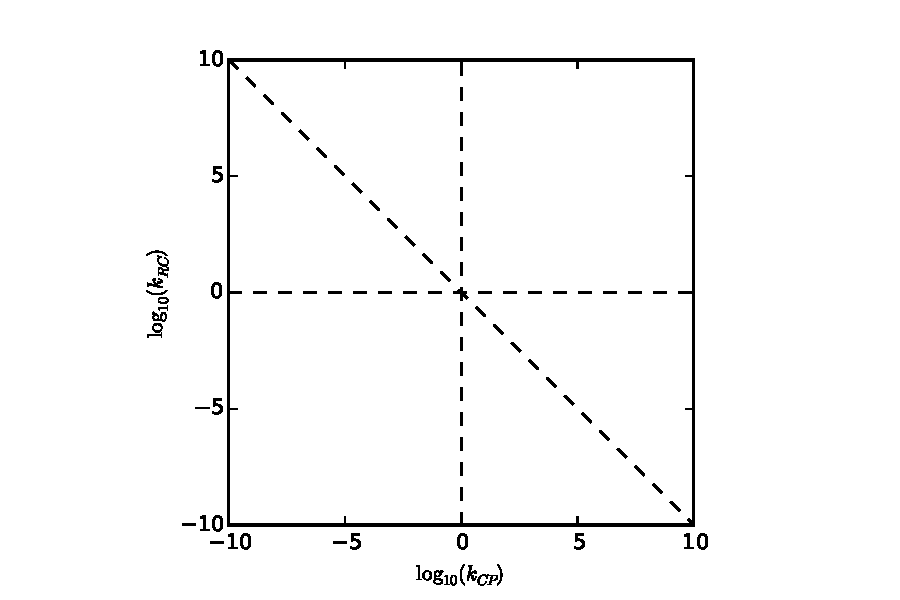
\includegraphics[scale=0.8]{C:/Users/Carlos/Documents/Tesis-IGP/code/Theory/ZonesSR.pdf}};

\node[circle,fill= blue!20,draw, minimum size=0.6cm,inner sep= 0] (R) at (-5.5,-4.5){R};
\node[circle,fill=blue!20,draw,minimum size=0.3cm, inner sep = 0] (C) at (-4.5,-3.8) {C};
\node[circle,fill=blue!20,draw,minimum size=1.cm,inner sep = 0](P) at (-5.5,-3.) {P};

 \path[every node/.style={font=\sffamily\small}]

(R) edge [<-,red] (C)
(R) edge [<-,red] (P)
(P) edge [->,red] (C);


\node[circle,fill= blue!20,draw, minimum size=0.3cm,inner sep= 0] (R) at (-4.5,-7.8){R};
\node[circle,fill=blue!20,draw,minimum size=0.6cm, inner sep = 0] (C) at (-3.5,-6.7) {C};
\node[circle,fill=blue!20,draw,minimum size=1.cm,inner sep = 0](P) at (-4.5,-5.6) {P};

 \path[every node/.style={font=\sffamily\small}]

(R) edge [<-,red] (C)
(R) edge [<-,red] (P)
(P) edge [->,red] (C);


\node[circle,fill= blue!20,draw, minimum size=1.cm,inner sep= 0] (R) at (-3.4,-3.6){R};
\node[circle,fill=blue!20,draw,minimum size=0.3cm, inner sep = 0] (C) at (-4.3,-2.6) {C};
\node[circle,fill=blue!20,draw,minimum size=0.6cm,inner sep = 0](P) at (-3.4,-2.1) {P};

 \path[every node/.style={font=\sffamily\small}]

(R) edge [<-,red] (C)
(R) edge [<-,red] (P)
(P) edge [->,red] (C);



\node[circle,fill= blue!20,draw, minimum size=1.cm,inner sep= 0] (R) at (-1.5,-4.1){R};
\node[circle,fill=blue!20,draw,minimum size=0.6cm, inner sep = 0] (C) at (-0.3,-3) {C};
\node[circle,fill=blue!20,draw,minimum size=0.3cm,inner sep = 0](P) at (-1.5,-2.1) {P};

 \path[every node/.style={font=\sffamily\small}]

(R) edge [<-,red] (C)
(R) edge [<-,red] (P)
(P) edge [->,red] (C);


\node[circle,fill= blue!20,draw, minimum size=0.6cm,inner sep= 0] (R) at (-0.1,-7){R};
\node[circle,fill=blue!20,draw,minimum size=1.0cm, inner sep = 0] (C) at (-1,-5.9) {C};
\node[circle,fill=blue!20,draw,minimum size=0.3cm,inner sep = 0](P) at (-0.1,-5.2) {P};

 \path[every node/.style={font=\sffamily\small}]

(R) edge [<-,red] (C)
(R) edge [<-,red] (P)
(P) edge [->,red] (C);


\node[circle,fill= blue!20,draw, minimum size=0.3cm,inner sep= 0] (R) at (-2.55,-7.8){R};
\node[circle,fill=blue!20,draw,minimum size=1.cm, inner sep = 0] (C) at (-1.8,-6.7) {C};
\node[circle,fill=blue!20,draw,minimum size=0.6cm,inner sep = 0](P) at (-2.55,-5.7) {P};

 \path[every node/.style={font=\sffamily\small}]

(R) edge [<-,red] (C)
(R) edge [<-,red] (P)
(P) edge [->,red] (C);


   
\end{tikzpicture}

  \caption{Divisi\'on del espacio $k_{\CP} \times k_{\RC}$ en funci\'on ah las relaciones de orden existentes entre las masas de las tres especies.}
\label{fig:ZonasSR}
\end{figure}
  






